\documentclass[12pt]{article}
\usepackage[utf8]{inputenc}
\usepackage[french]{babel}
\usepackage{hyperref}
\usepackage{listings}
\usepackage{color}
\usepackage{graphicx}
\usepackage{titlesec}
\usepackage{caption}
\usepackage{geometry}
\usepackage{float}
\geometry{margin=2.5cm}

\definecolor{codegray}{rgb}{0.95,0.95,0.95}
\lstset{
  backgroundcolor=\color{codegray},
  basicstyle=\ttfamily\small,
  frame=single,
  breaklines=true
}

\title{\textbf{}}
\author{}
\author{}
\date{}

\begin{document}
% Page de garde
\begin{titlepage}
    \centering
    \vspace*{1cm}
    
    % LOGO de l'institut
    
\includegraphics[width=7cm]{captures/285806862_133769749266390_5860943595045476590_n.jpg}\\[1cm] % <-- Remplace "logo.png" par le nom exact de ton fichier image

    {\Large \textbf{INSTITUT NATIONAL SUPÉRIEUR D’INFORMATIQUE}}\\[1cm]

    {\LARGE \textbf{Configuration d'un système de détection et de prevention avec Snort}}\\[2cm]

    \begin{flushleft}
        \textbf{MENTION :} Informatique\\[0.5cm]
        \textbf{PARCOURS :} ARSB\\[0.5cm]
        \textbf{ANNÉE UNIVERSITAIRE :} Licence 2 – 2024–2025\\[0.5cm]
        \textbf{RÉALISÉ PAR :}\\
        LAHINIRIKO Mara Sylvain\\
        MBOLANIRINA Stephano Kevin
    \end{flushleft}

    \vfill
\end{titlepage}
\maketitle

\section*{Introduction}

Dans le domaine de la sécurité réseau, \textbf{Snort} est un outil incontournable pour détecter et analyser les intrusions en temps réel. Open source et largement utilisé, il permet de surveiller le trafic réseau et de repérer toute activité suspecte grâce à des règles personnalisées.

Dans ce premier guide, d’autres vont suivre, je vais vous montrer comment installer, configurer et utiliser \textbf{Snort} pour détecter les intrusions. Nous aborderons également la création de règles personnalisées et l’analyse des alertes générées pour agir rapidement en cas d’incident.

\section{C’est quoi Snort ?}

\textbf{Snort} est un logiciel de \textbf{détection d’intrusion réseau (NIDS)} reconnu pour sa capacité à surveiller et protéger les réseaux informatiques en temps réel.

Il fonctionne selon plusieurs modes :
\begin{itemize}
  \item \textbf{Mode sniffer} : capture le trafic réseau en temps réel.
  \item \textbf{Mode enregistreur de paquets} : enregistre les paquets pour analyse ultérieure.
  \item \textbf{Mode IDS} : compare les paquets réseau à des règles prédéfinies et génère des alertes.
\end{itemize}

\section{Un peu d’histoire}

Depuis sa création en 1998 par \textbf{Martin Roesch}, Snort a évolué pour devenir l’un des outils NIDS les plus utilisés. Initialement simple capteur de paquets, il a intégré des fonctions avancées avec le temps.

En 2013, \textbf{Cisco Systems} a acquis Sourcefire, la société à l’origine de Snort, renforçant son développement et son intégration dans les systèmes professionnels.

\section{Installation de Snort}

Nous allons installer la version 3.5.0 de Snort sur une machine Debian 12(elle fonctionne également sur une Ubuntu 24.04), cette machine est ma machine de rebonds de mon homelab.

\subsection*{Étape 1 : Préparation de l’environnement}

Commencez par mettre à jour votre système pour vous assurer que tous les paquets sont récents et compatibles avec l’installation.

\begin{lstlisting}[language=bash]
sudo -i
apt update && apt upgrade -y
\end{lstlisting}

Ensuite, installez les dépendances essentielles pour compiler et exécuter Snort 3.5.0 :
\begin{lstlisting}[language=bash]
apt install -y git wget build-essential libpcap-dev libpcre3-dev \
libdumbnet-dev zlib1g-dev libluajit-5.1-dev libssl-dev cmake libunwind-dev \
luajit hwloc bison flex liblzma-dev openssl pkg-config libhwloc-dev \
cpputest libsqlite3-dev uuid-dev libcmocka-dev libnetfilter-queue-dev \
libmnl-dev autotools-dev libfl-dev libgoogle-perftools-dev ethtool
\end{lstlisting}

\subsection*{Étape 2 : Installation de DAQ (Data Acquisition Library)}

\textbf{DAQ} est une bibliothèque indispensable pour \textbf{Snort} puisqu’elle gère la capture de paquets. DAQ permet à \textbf{Snort} de fonctionner avec plusieurs moteurs de capture comme \textbf{pcap} ou \textbf{afpacket}.

1.Clonez le dépôt DAQ :
\begin{lstlisting}[language=bash]
git clone https://github.com/snort3/libdaq.git\end{lstlisting}

2.Configurez, compilez et installez DAQ :
\begin{lstlisting}[language=bash]
cd libdaq
./bootstrap
./configure
make
sudo make install
ldconfig
\end{lstlisting}

\textbf{DAQ} est maintenant installé et prêt à être utilisé comme bibliothèque de capture pour \textbf{Snort}.

\subsection*{Étape 3 : Installation de Snort 3.5.0}

1.Téléchargez Snort 3.5.0 depuis le site officiel :
\begin{lstlisting}[language=bash]
cd ..
wget https://github.com/snort3/snort3/archive/refs/tags/3.5.0.0.tar.gz
\end{lstlisting}

2.Extrayez l’archive :
\begin{lstlisting}[language=bash]
tar -xzvf 3.5.0.0.tar.gz
cd snort3-3.5.0.0
\end{lstlisting}

3.Configurez \textbf{Snort} en incluant les options pour \textbf{gperftools} et DAQ
\begin{lstlisting}[language=bash]
./configure_cmake.sh --prefix=/usr/local --enable-tcmalloc
\end{lstlisting}

.Compilez et installez \textbf{Snort} :
\begin{lstlisting}[language=bash]
cd build
make
make install
ldconfig
\end{lstlisting}

5.Vérifiez l’installation de \textbf{Snort} :
\begin{figure}[H] 
    \centering
    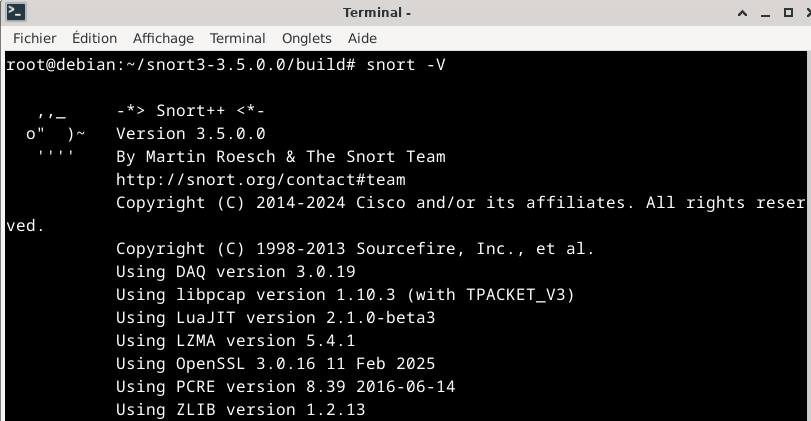
\includegraphics[width=0.8\textwidth]{captures/Pasted image 20250603104154.png}
    \label{fig:mon_image}
\end{figure}

\vspace{0.5cm}
\noindent Snort est maintenant installé et prêt à être configuré et utilisé pour la détection d’intrusions réseau.

\section{Configuration de l’interface réseau}

Pour que Snort capture tous les paquets, l’interface réseau doit être placée en \textbf{mode promiscuous}.Cette configuration est essentielle pour un système de détection d’intrusion, car elle permet de capturer tous les paquets qui passent par l’interface, même ceux qui ne lui sont pas directement destinés. Voyons en détail ce qu’est le mode promisc et comment l’activer pour une interface réseau, ici `enp1s0`.

\subsection*{Qu’est-ce que le mode PROMISC ?}

En mode normal, une carte réseau traite seulement les paquets qui lui sont adressés. En mode \textbf{promiscuous}, elle capte tout le trafic transitant sur le réseau, même non destiné à sa propre adresse.

\subsection*{Configuration de l'interface}
Sous Linux, il est simple d’activer le mode promisc pour une interface réseau en utilisant des commandes comme ip ou \textbf{ifconfig}. Voici les étapes pour activer ce mode pour l’interface `enp1s0`. Remplacez le nom de l’interface réseau en fonction de votre configuration.

Par ailleurs, pour éviter que Snort ne tronque les paquets volumineux, nous devons désactiver certaines fonctions d’offloading au niveau de l’interface réseau. Ces fonctions sont souvent activées par défaut pour améliorer les performances du réseau, mais elles peuvent interférer avec la capture de paquets complète requise par Snort.

\subsection*{Étape 1 : Activer le mode promiscuous}

1. Pour activer le mode promiscuous sur l’interface réseau `enp0s8`, exécutez la commande suivante :
\begin{lstlisting}[language=bash]
sudo ip link set enp1s0 promisc on
\end{lstlisting}

Pour vérifier l’état :

\begin{figure}[H] % H = ici exactement, nécessite le package float
    \centering
    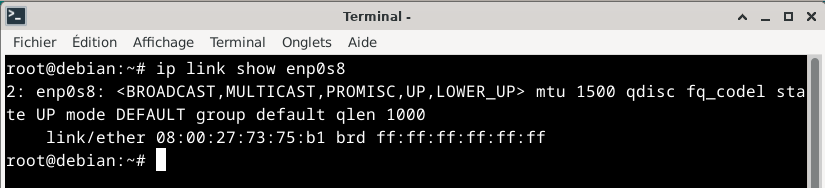
\includegraphics[width=0.8\textwidth]{captures/Pasted image 20250604070119.png}
    \label{fig:mon_image}
\end{figure}


\subsection*{Étape 2 : Désactiver l’Interface Offloading}

L’Interface \textbf{Offloading} est une série d’optimisations matérielles utilisées pour décharger le traitement des paquets vers la carte réseau, ce qui peut réduire la charge CPU. Cependant, ces options peuvent causer des problèmes avec \textbf{Snort}, notamment en tronquant les paquets de plus de 1518 octets, ce qui empêche \textbf{Snort} de capturer certaines menaces de manière complète.

Pour éviter les paquets tronqués, désactiver GRO et LRO :

\begin{lstlisting}[language=bash]
ethtool -K enp1s0 gro off
ethtool -K enp1s0 lro off
\end{lstlisting}

Vérification :

\begin{figure}[H] % H = ici exactement, nécessite le package float
    \centering
    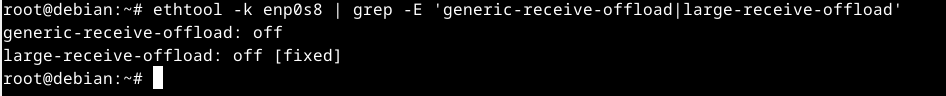
\includegraphics[width=0.8\textwidth]{captures/Pasted image 20250604080003.png}
    \label{fig:mon_image}
\end{figure}


\noindent Cela garantit que Snort capture les paquets dans leur intégralité, même au-delà de 1518 octets.

\subsection*{Étape 3 : Rendre les changements permanents}
Le but est créer deux scripts, un pour l'IDS et un pour l'IPS mais aussi les services corréspondants.

\subsubsection*{1-Configuration de l' IDS}
Voici le script qui fait le lancement du service IDS. Ce script doit être stocké dans le répertoire \textbf{/usr/local/bin/} et nommé \textbf{run\_snort\_ids.sh}
\begin{figure}[H] % H = ici exactement, nécessite le package float
    \centering
    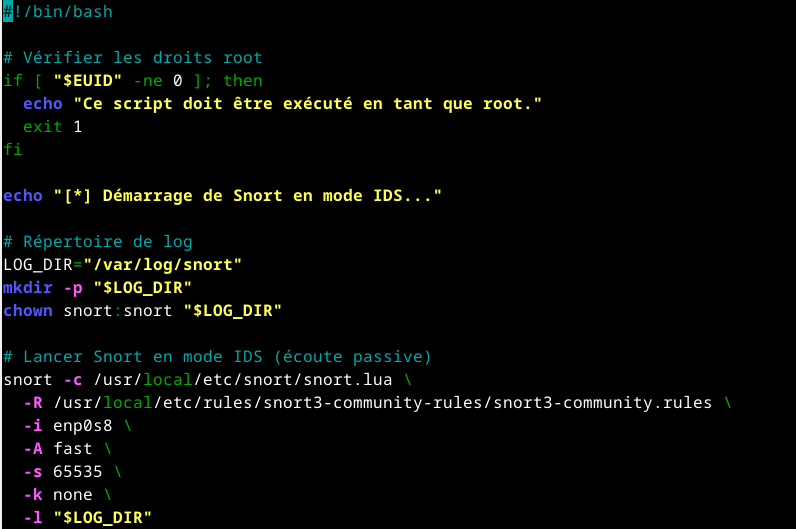
\includegraphics[width=0.8\textwidth]{captures/image1.png}
    \label{fig:mon_image}
\end{figure}
Ce script doit être éxecuté en tant que\textbf{root}.\\
\begin{itemize}
    \item \textbf{LOGDIR="/var/log/snort}: c'est dans ce repertoire ques les logs de capture de paquets seront enregistré
    \item la dérnière section permet de lancer snort en mode IDS
\end{itemize}

\paragraph{Création du service IDS:}
Pour que le scrit soit lancer automatiquement à chaque redémarrage, nous avons de créer un service permettant de le faire. Ce service doit impérativement être stocké dans le répertoire : \textbf{/etc/sytemd/system/}, on va le nommé : \textbf{snort-ids.service}. Le contenu du fichier \textbf{service} est affiché ci-dessous
\begin{figure}[H] 
    \centering
    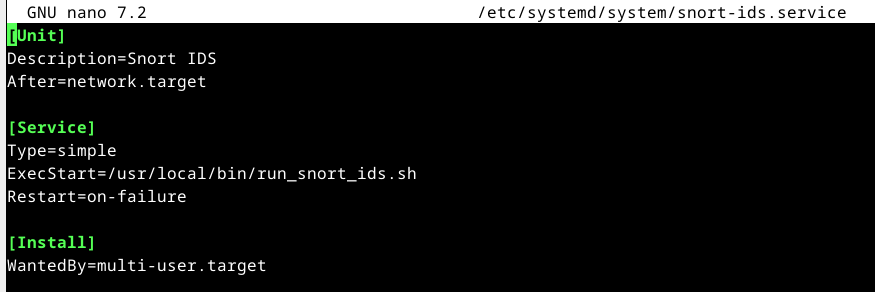
\includegraphics[width=0.8\textwidth]{captures/image3.png}
    \label{fig:mon_image}
\end{figure}

\subsubsection*{2-Configuration de l' IPS}
Voici le script qui fait le lancement du service IPS. Ce script doit être stocké dans le répertoire \textbf{/usr/local/bin/} et nommé \textbf{run\_snort\_ips.sh}
\begin{figure}[H] 
    \centering
    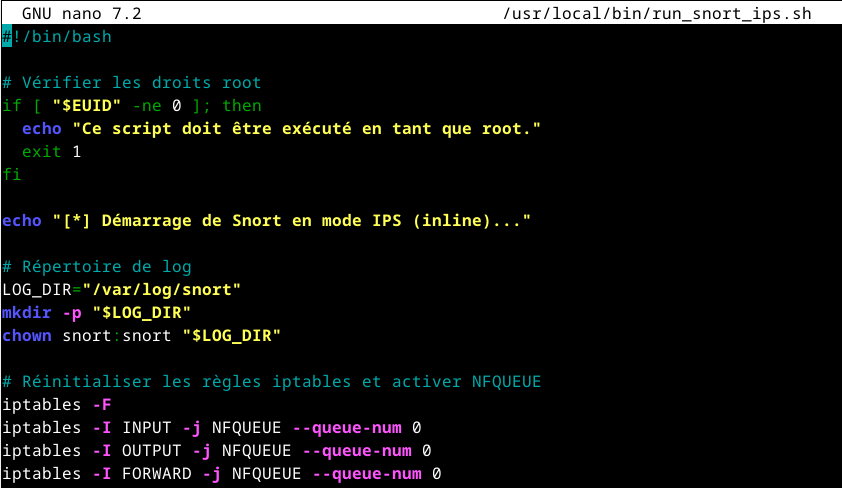
\includegraphics[width=0.8\textwidth]{captures/image4.png}
    \label{fig:mon_image}
\end{figure}
\begin{figure}[H] % H = ici exactement, nécessite le package float
    \centering
    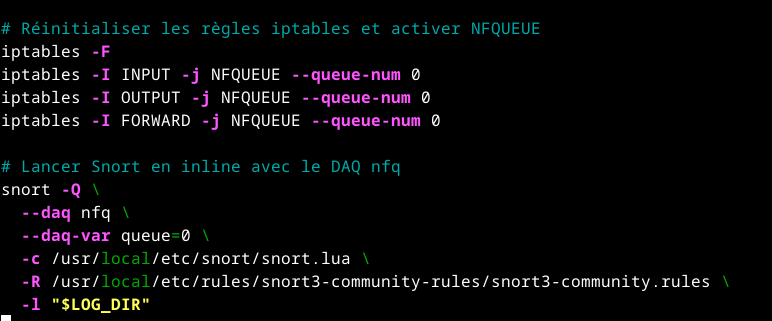
\includegraphics[width=0.8\textwidth]{captures/image5.png}
    \label{fig:mon_image}
\end{figure}
Ce script doit être éxecuté en tant que \textbf{root}.\\
\begin{itemize}
    \item \textbf{LOGDIR="/var/log/snort}: c'est dans ce repertoire ques les logs de capture de paquets seront enregistré
    \item les règles iptables doivent être réinitialisées et activées l'outil NFQUEU pour que snort prevenir lorsqu'il y a des attaques.

    \item le dernière section permet snort en mode IPS.
\end{itemize}
\paragraph{Création du service IDS:}
Pour que le script de l'IPS soit lancer automatiquement aussi à chaque redémarrage, nous allons crée un service permettant de le faire. Ce service doit impérativement être aussi stocké dans le répertoire : \textbf{/etc/sytemd/system/}, on va le nommé : \textbf{snort-ips.service}. Le contenu du fichier \textbf{service} est affiché ci-dessous
\begin{figure}[H] 
    \centering
    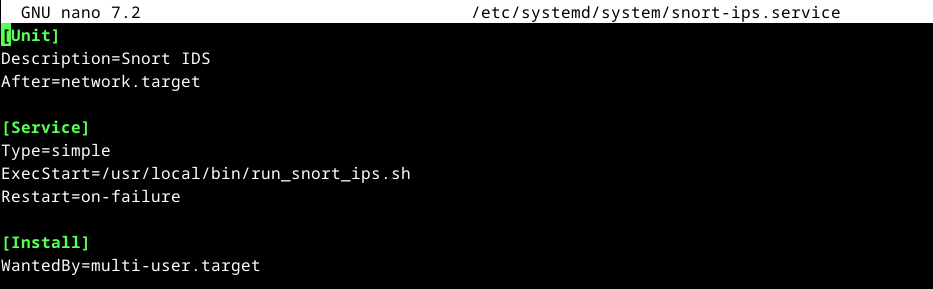
\includegraphics[width=0.8\textwidth]{captures/image2.png}
    \label{fig:mon_image}
\end{figure}
Activez ensuite les services pour qu’il démarre automatiquement :
\paragraph{Activation de service IDS}

\begin{lstlisting}[language=bash]

sudo systemctl enable snort-ids.service
sudo systemctl start snort-ids.service
\end{lstlisting}
\begin{figure}[H] 
    \centering
    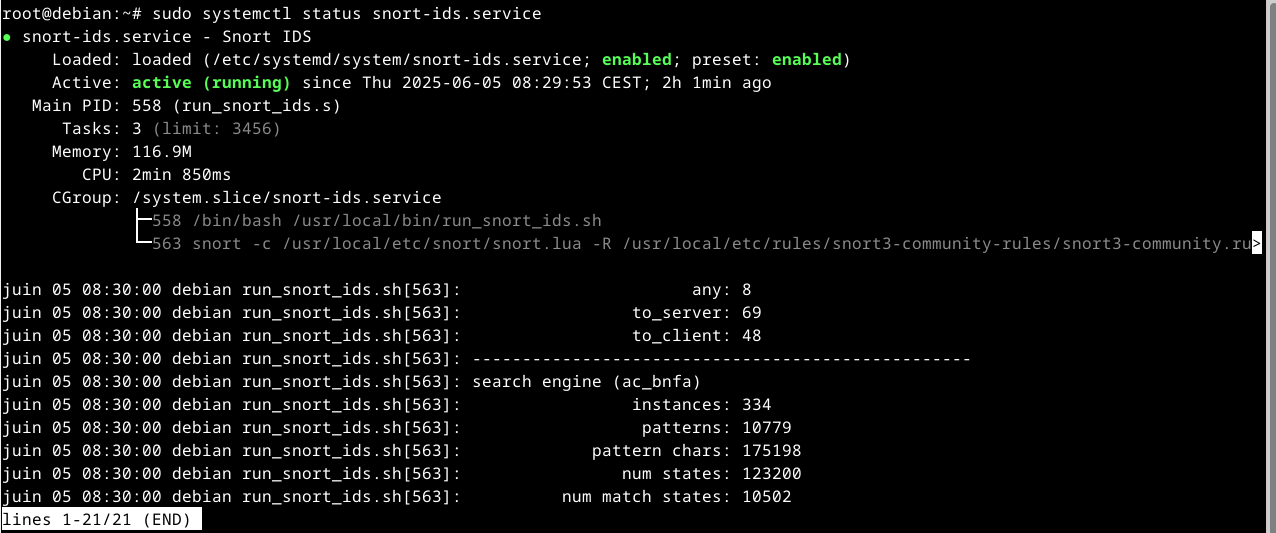
\includegraphics[width=0.8\textwidth]{captures/image6.png}
    \label{fig:mon_image}
\end{figure}
\paragraph{Activation de service IPS}

\begin{lstlisting}[language=bash]

sudo systemctl enable snort-ips.service
sudo systemctl start snort-ips.service
\end{lstlisting}
\begin{figure}[H] 
    \centering
    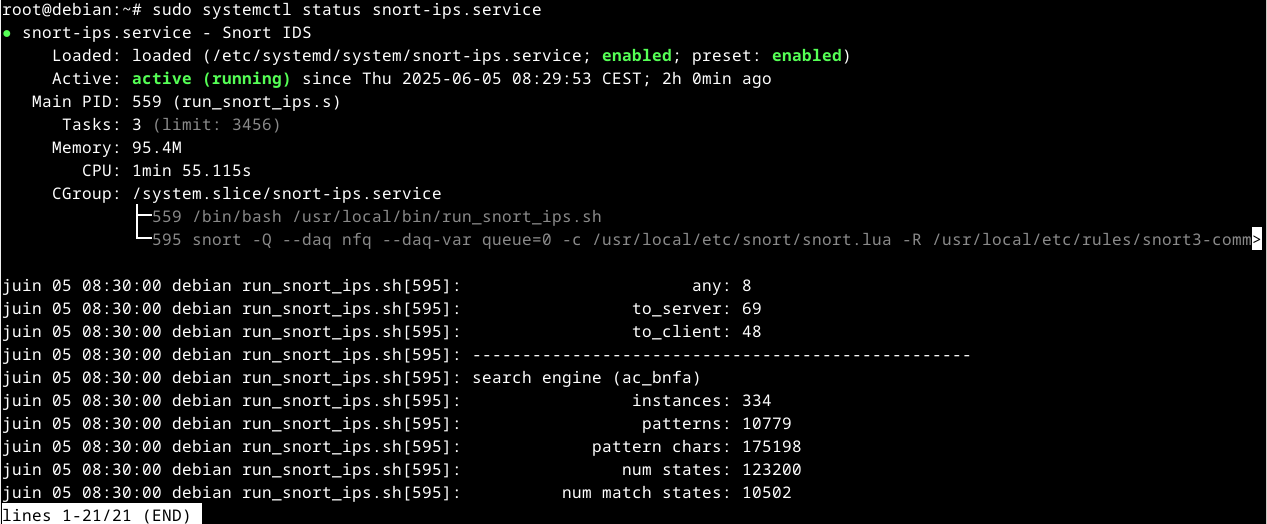
\includegraphics[width=0.8\textwidth]{captures/image7.png}
    \label{fig:mon_image}
\end{figure}

\section{Configuration de base de Snort}
Après avoir installé \textbf{Snort 3.5.0} avec toutes les dépendances, la prochaine étape est la configuration initiale pour que \textbf{Snort} puisse analyser le trafic réseau efficacement. Le fichier de configuration principal de \textbf{Snort} est \textit{snort.lua} (au lieu de snort.conf dans les versions précédentes). Nous allons voir comment configurer \textbf{Snort} pour surveiller une interface spécifique, ici \textbf{enp0s8} et comment définir les paramètres de base.

\subsection{Étape 1 : Ouvrir et éditer le fichier de configuration}
Le fichier de configuration par défaut pour \textbf{Snort 3 }est un fichier Lua généralement situé dans /usr/local/etc/snort/snort.lua. Commencez par ouvrir ce fichier dans un éditeur de texte :

\begin{lstlisting}[language=bash]
sudo nano /usr/local/etc/snort/snort.lua
\end{lstlisting}
\subsection{Étape 2 : Configurer l’interface réseau}
Dans le fichier de configuration, spécifiez l’interface réseau à surveiller. Dans ce cas, nous utiliserons \textbf{enp0s8} comme interface pour capturer le trafic.
\subsubsection{Localisez la section qui définit l’interface réseau et modifiez-la pour qu’elle pointe vers enp0s8 :}

\begin{lstlisting}[language=bash]
##interface a surveiller
interface = "enp0s8"
\end{lstlisting}
\subsubsection{Cette interface sera maintenant surveillée en continu par Snort, permettant de capturer tout le trafic entrant et sortant sur cette interface.}

\subsection{Étape 3 : Définir les réseaux surveillés et externes}
Pour que Snort puisse distinguer le trafic local du trafic externe, il est essentiel de définir les variables HOME\_NET et EXTERNAL\_NET dans le fichier snort.lua. Cela aide Snort à générer des alertes spécifiques au réseau surveillé.
\subsubsection{Dans la section des variables réseau, configurez les valeurs pour HOME\_NET et EXTERNAL\_NET. Par exemple :}

\begin{lstlisting}[language=bash]
HOME_NET = '192.168.63.0/24'
EXTERNAL_NET = 'any'
\end{lstlisting}
\paragraph{HOME\_NET : définit le sous-réseau local (remplacez 192.168.63.0/24 par votre réseau local).
}
\paragraph{EXTERNAL\_NET : any signifie que tout ce qui n’est pas dans HOME\_NET sera considéré comme externe.
}
\subsection{Étape 6 : Activer les règles de détection}
Les règles de détection permettent à Snort d’identifier les menaces. En fonction de votre environnement, vous pouvez activer des règles spécifiques dans le fichier snort.lua :

\subsubsection{Incluez les fichiers de règles nécessaires pour analyser les menaces. Si vous avez téléchargé des règles, comme les règles de base ou les règles communautaires de Snort, assurez-vous de spécifier leur emplacement dans snort.lua :}

\begin{lstlisting}[language=bash]
ips =
{
-- use this to enable decoder and inspector alerts
enable_builtin_rules = true,
include = RULE_PATH .. "/local.rules",
-- use include for rules files; be sure to set your path
-- note that rules files can include other rules files
-- (see also related path vars at the top of snort_defaults.lua)
variables = default_variables
}
\end{lstlisting}

Ici le fichier des règles se trouve sur le repertoire /usr/local/etc/rules/ c'est qui est remplacé par RULE\_PATH

ET pour les règles, on a téléchargé de fichier rules dans le site officielles de snort et on a copier sur le fichier local.rules qui est notre fichier personnelle.
\section{Test simple}
Une fois que Snort est installé et configuré, il est essentiel de tester son bon fonctionnement pour s’assurer qu’il détecte bien les événements réseau. Un test simple consiste à utiliser la commande ping depuis une autre machine pour générer un type de trafic réseau courant. Cette opération permettra de vérifier que Snort capture les paquets ICMP (Internet Control Message Protocol) et génère une alerte en conséquence.

Dans cette teste, on va faire une teste  de surveiller le trafic ICMP et à générer des alertes lorsqu’il détecte un ping.

On a trois machines : le premier machiene est le system de defence lequelle snort est installé , le deuxième machine est la machine cible pour simuler une attaque et le dernier machine est une machine hôte parce que le réseau que nous allons surveiller est le réseau d'une téléphone.

\textit{on va lance une ping sur le PC hôte vers le PC cible }
\begin{figure}[H] 
    \centering
    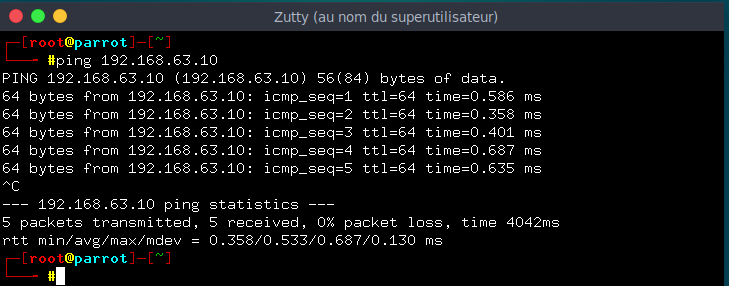
\includegraphics[width=0.8\textwidth]{captures/image9.png}
    \label{fig:mon_image}
\end{figure}
On va verifié le fichier log depuis le machine system de défence et On voit les messages de ping avec protocole ICMP suivant dans le fichier alert\_fast.txt :
\begin{figure}[H] 
    \centering
    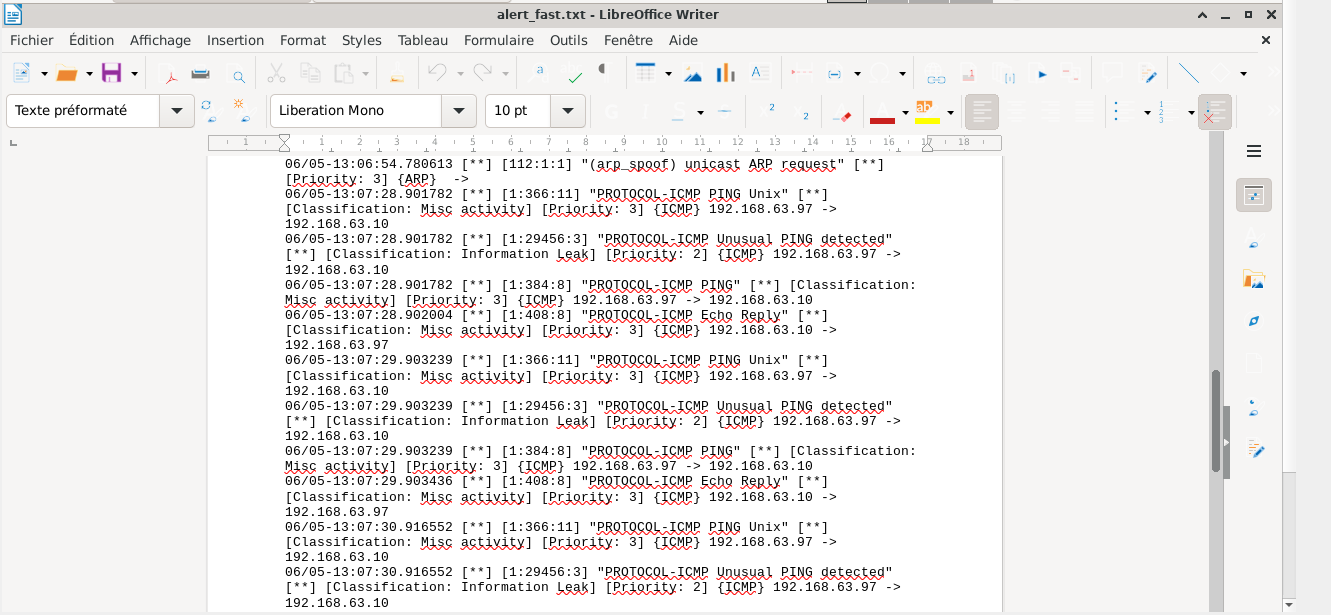
\includegraphics[width=0.8\textwidth]{captures/image8.png}
    \label{fig:mon_image}
\end{figure}

\section*{Conclusion}

Ce guide a présenté les étapes essentielles pour la mise en place d’un système de détection et de prévention d'intrusion (IDS/IPS) à l’aide de Snort 3.5.0 sur une distribution Debian 12. En partant de l’installation des dépendances jusqu’à la configuration du service et de la capture de trafic via NFQUEUE, nous avons mis en œuvre un système capable d’analyser  les paquets qui circulent sur l’interface réseau.

Cette configuration constitue une base solide pour surveiller et protéger un réseau contre des menaces connues. Toutefois, afin d'assurer une sécurité optimale, il est recommandé d’enrichir continuellement les règles Snort, de maintenir le système à jour, et d’intégrer cette solution à un ensemble d’outils de sécurité plus large dans le cadre d’une politique de défense en profondeur.

\end{document}
